\chapter{Glossar}
\section{HTML [FK]}\label{sec:HTML}
HTML bedeutet „Hypertext Markup Language“. Mit HTML kann man Dokumente strukturieren und Bilder sowie auch Hyperlinks einfügen. HTML Dokumente sind die Grundlage des Internets. Jede Website basiert darauf. (vgl. \cite{HTML})
\section{CSS [FK]}\label{sec:CSS}
CSS bedeutet „Cascading Style Sheets “. Damit können Dokumente wie HTML Grafikmäßig angepasst werden. Somit kann jeder Text, jeder Knopf, jede Fläche anders positioniert und gefärbt werden. Es gehört ebenfalls wie HTML zu den Grundlagen des Internet und wird in jeder Website verwendet. (vgl. \cite{CSS})
\section{SVG [FK]}\label{sec:SVG}
SVG bedeutet „Scalable Vector Graphics“.SVG ist die vom World Wide Web Consortium (W3C) empfohlene Spezifikation zur Beschreibung zweidimensionaler Vektorgrafiken. SVG, das auf XML basiert, wurde erstmals im September 2001 veröffentlicht. Praktisch alle relevanten Webbrowser können einen Großteil des Sprachumfangs darstellen. (vgl \cite{SVG})
\section{AD und LDAP [FK]}\label{sec:AD}
AD bedeutet Active Directory. Das Active Directory ist als Verzeichnisdienst eine der zentralen Komponenten zur Verwaltung von Windows-basierten Netzwerken. Im Verzeichnis sind die verschiedenen Geräte und Ressourcen eines Netzwerks inklusive ihrer Attribute gespeichert.
Mit Hilfe des Active Directories lässt sich die Struktur des Netzwerks mit seinen angeschlossenen Geräten der Struktur einer Organisation nachbilden. Einzelne Unternehmensbereiche sind über so genannte Domänen voneinander abgegrenzt.
Die Domänen können hierarchisch gegliedert sein. Über das Active Directory kann nach bestimmten Geräten oder Attributen gesucht werden. Dem Administrator ermöglicht das AD die zentrale Verwaltung der Benutzerrechte für einzelne Geräte oder Objekte. Netzwerkressourcen lassen sich für Anwender freischalten oder sperren. Schreibenden Zugriff auf den Verzeichnisdienst erhalten daher in der Regel nur die Administratoren des Netzwerks.
Zu den administrierbaren Ressourcen zählen unter anderem Speicherplatz, Zugriffsrechte auf Verzeichnisse, Nutzungsrechte von Anwendungen, Netzwerkdrucker, Peripheriegeräte und andere Netzwerkdienste. (vgl. \cite{AD})
LDAP bedeutet Lightweight Directory Access Protocol. Es ermöglicht Abfragen an das AD System. (vgl. \cite{LDAP}
\section{Hyper-V [FK]}\label{Hyper-V}
Hyper-V ist die Windows Server Virtualisierung. Damit ist es in Windows möglich Virtuelle Maschinen zu erzeugen. Dieses Feature ist in den neueren Windows Server Versionen Standardmäßig installiert. In den Clientbetriebssystemen ist dies nur in den Enterprise und Pro Versionen von Windows 8 und 10 verfügbar. Mit Hyper-V kann man komplett vom restlichen Betriebssystem Isolierte Systeme erstellen.
vgl. (vgl. \cite{Hyper-V})
\section{API [FK]}\label{sec:API}
API bedeutet „Application Programming Interface “. Auf Deutsch ist damit eine Programmierschnittstelle gemeint mit der man Zugriff auf Daten von einem System erhält. Eine API wird benötigt um einen klaren Punkt zu definieren an dem man die benötigten Daten abholen kann sofern man die Berechtigung dazu hat. (vgl. \cite{API})
\section{CMD [FK]}\label{sec:CMD}
CMD bedeutet „Command“. Gemeint ist damit die Windows Eingabeaufforderung auch genannt Terminal. In dieser Arbeit verwende ich den Begriff CMD allgemein für Kommandozeilenbefehle egal ob auf Windows oder Linux basierten Systemen. Mit Terminals können alle möglichen Befehle auf einem Rechner ausgeführt werden. Somit sind Terminals ein sehr Wertvolles Werkzeug speziell für Server welche meistens kein Grafisches Benutzerinterface besitzen. (vgl. \cite{CMD})
\begin{figure}[H]
    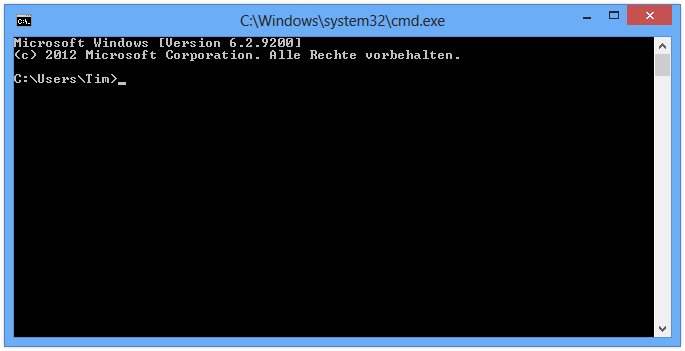
\includegraphics[scale=0.8]{images/cmdExample.png}
    \caption{CMD Beispiel}
    \label{img:cmdExample}
    \url{https://upload.wikimedia.org/wikipedia/de/4/48/Cmd_in_Windows_8.png}
\end{figure}
\section{JSON [FK]}\label{sec:json}
JSON bedeutet „JavaScript Object Notation “. JSON ist ein Dateiformat mit dem Hauptsächlich Daten Übertragen werden. Es ist gut zum Transferieren von Daten, weil es ein einfaches Schema besitzt und auf Stylings (wie in HTML) verzichtet. Das Schema besteht lediglich aus Objekten welche mit einer geschwungenen Klammer markiert werden. In diesen Objekten werden Key-Value Daten gespeichert. Der Wert (Value) kann aber auch ein anderes Objekt (geschachteltes Objekt) oder ein Array von Werten oder wieder Objekten sein. (vgl. \cite{JsonVsXml})
\begin{figure}[H]
    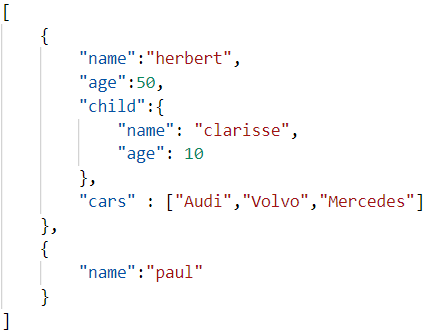
\includegraphics[scale=1]{images/jsonExample.PNG}
    \caption{JSON Beispiel}
    \label{img:jsonExample}
\end{figure}
\section{XML [FK]}\label{sec:xml}
XML bedeutet „Extensible Markup Language“. XML ist ebenfalls wie JSON ein Format um Daten zu übertragen aber bei XML wird deutlich mehr Wert auf die Hierarchie und die Strukturierung gelegt. Somit wird das Dokument zwar für Menschen leichter lesbar aber auf kosten der Geschwindigkeit beim Lesen der Daten. (vgl. \cite{JsonVsXml})
\section{Index [FK]}\label{sec:Index}
Ein Index existiert um die Abfragegeschwindigkeit von Datenbankabfrage zu beschleunigen. In der Indextabelle werden die Daten sortiert gespeichert. Ein Index selbst ist eine Art Zeiger der auf den ausgesuchten Datensatz zeigt. Ein Index ist besonders effektiv bei großen Datenmengen welche sehr oft benötigt werden. Es sollte aber nicht auf jeden Datensatz ein Index angelegt werden denn auch wenn es nur ein Zeiger ist verbraucht es Speicherplatz der bei vielen Indizes stark ansteigen kann. Bei Änderungen auf den Daten müssen außerdem die Indizes angepasst werden. (vgl. \cite{Index})
\section{JDBC [FK]}\label{sec:JDBC}
JDBC bedeutet “Java Database Connectivity”. JDBC ist die Schnittstelle von Java Programmen zu den verschiedenen Datenbanken. Es gibt somit eine einheitliche Schnittstelle um auf alle relationalen Datenbaken zugreifen zu können. (vgl. \cite{JDBC})
\section{VM [FK]}\label{sec:VM}
VM bedeutet „Virtual Machine“. Eine VM ist eine abgekapselte Version eines Computers. Die VM versucht die Hardware eines real existierenden Computers nachzustellen. Es können somit mehrere Instanzen auf derselben Hardware laufen ohne sich gegenseitig zu beeinflussen. Der Unterschied zu Emulatoren ist das Emulatoren ein System rein mit Software nachstellen und VMs direkt auf die Hardware zugreift. (vgl. \cite{VM})
\section{Node [FK]}\label{sec:Node}
Nodes sind bei verteilten Systemen die einzelnen Computersysteme die verbunden sind. 
\section{DNS [FK]}\label{sec:DNS}
DNS bedeutet „Domain Name System“. Wenn ein Benutzer auf eine bestimmte Website gelangen will kann er einfach den Namen (Domain) der Website eingeben und er kommt auf die gewünschte Seite. Computer verstehen diese Namen aber nicht direkt sie reagieren nur auf IP-Adressen (z.b. 192.56.5.23) der DNS wandelt nun die Textanfrage des Benutzers auf die zugehörige IP um. (vgl. \cite{DNS})
\section{Nginx [FK]}\label{sec:nginx}
Nginx ist ein Webserver. Der Webserver kann verwendet werden um alle möglichen Webseiten zu Hosten. Nginx kann außerdem als Email Server und Reverse Proxy verwendet werden. (vgl. \cite{Nginx})
\section{DOM [FK]}\label{sec:dom}
DOM bedeutet „Document Object Model“. Das DOM enthält alle Objekte die auf einer Website existieren. Es ist Programmiersprachen unabhängig was es ermöglicht eine Website einfach zu verändern. Durch diese Wandlungsfähigkeit werden dynamische Webseiten ermöglicht. (vgl. \cite{DOM})